\chapter{Physics}\label{ch:physics}

\begin{wrapfigure}{R}{0.3\textwidth}
    \centering
    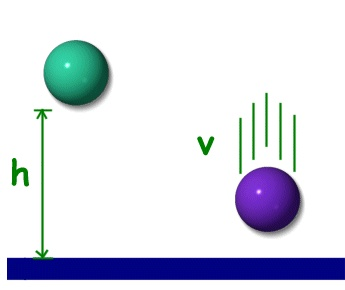
\includegraphics[width=0.25\textwidth]{images/physics}
\end{wrapfigure}

Physics is a huge and fascinating science, dealing with the big (astronomy, astrophysics), the small (nuclear and particle physics), the universal (electromagnetism, thermodynamics) and the more complicated (quantum physics, relativity); basically how the universe behaves, or at least how matter moves through space and time as well as energy and force.

For our purpose though, we will focus on \textbf{classical physics}, mechanics to be precise and its sub-branches, the fundamental concepts of time, space and how they give rise to higher phenomena encountered during CI, and we won't go into the realm of quantum physics as this is beyond the human perception and not of any use to us.
An understanding of physics isn't really needed though --in order to use it, to play with it-- as it doesn't really help on a perceptual/experiential, bodily level.

In CI we engage in the exploration of physics, to play with physical forces, with the direction of movement and its changes in space.
It might be interesting though to see what you learned in physics, to see what's yet \textbf{embodied}.
Engineers might smile hearing terminology from the world of leverage, friction, mutual point of contact, center of mass and so on.
Preferably after that chapter you are also familiar with terms such as: gravity, vector, inertia, force, momentum, and kinetics.

\section{Energy}\label{sec:energy}

The word ``energy'' is just too often misused in the spiritual world as some metaphysical, psycho-telepathic \textbf{mystery}.
In physics, we define it simply as ``\textit{the capacity for doing work}'', and as such different forms exist: potential (position), kinetic (movement), thermal (heat), nuclear (atom), electrical (charges), chemical, and so on.
All forms of energy are associated with motion: Any given body has kinetic energy if it's in motion.
A tensioned device such as a bow, a spring, or your tendons, though at rest, have the potential for creating motion; it contains potential energy.
Energy can neither be created nor destroyed, but only transformed from one form to another, which is stated in the first law of thermodynamics: energy conservation.

\section{Mechanics}\label{sec:mechanics}

Here we are interested in the relationship between force, matter and motion, as seen from a Newtonian perspective, focusing on motion (\textbf{kinematics} or ``\textit{the geometry of motion}'') and forces (\textbf{dynamics}).

Newton's laws of motion (classical mechanics) state:

\begin{enumerate}
    \item ``\textit{A body remains at rest, or in motion at a constant speed in a straight line, except insofar as it is acted upon by a force.}'' \\
    This law expresses the principle of \textbf{\gls{inertia}}: the natural behavior of a body is to move in a straight line at constant speed. \\
    A body's motion preserves the status quo, but external forces can disturb this.
    \item ``\textit{The net force on a body is equal to the body's instantaneous acceleration multiplied by its instantaneous mass or, equivalently, the rate at which the body's momentum changes with time.}'' ($F = ma$) \\
    This law is about motion, or as we call it nowadays \textbf{\gls{momentum}}. \\
    It depends upon the amount of matter contained in a body, the speed at which that body is moving, and the direction in which it is moving. \\
    In modern notation, the momentum of a body is the product of its mass and its velocity. \\
    The forces acting on a body add as \textbf{\gls{vector}s}: Quantities with both magnitude (amount of motion) and direction (of motion). \\
    So the total force on a body depends upon both the magnitudes and the directions of the individual forces. \\
    When the net force on a body is equal to zero, then by Newton's second law, the body does not accelerate, and it is said to be in \textbf{mechanical equilibrium}. \\
    Momentum is conserved in a closed system, meaning that the total momentum before an event --such as a collision-- is equal to the total momentum after the event, as long as no external forces are acting on the system.
    \item ``\textit{To every action, there is always opposed an equal reaction; or, the mutual actions of two bodies upon each other are always equal, and directed to contrary parts.}'' \\
    This relates to the conservation of momentum.
\end{enumerate}

Further candidates for \textbf{additional laws} are:
\begin{enumerate}
    \item \textit{Uniformly accelerated motion}, also known as: \textbf{free fall}. \\
    When a body falls (in the absence of air resistance), it will accelerate at a constant rate. \\
    The speed with which it falls is proportional to the elapsed time, and the acceleration is the same for all bodies, independent of their mass (``\textit{law of universal gravitation}'').
    \item \textit{Uniform circular motion}, which contains the \textbf{centripetal} force and is required to sustain the acceleration towards the center. \\
    The \textbf{centrifugal} force is, on the other hand, an inertial (fictitious/pseudo) force that is directed radially away from the axis of rotation.
    \item \textit{Harmonic motion}, as shown by a spring-mass system or a pendulum.
\end{enumerate}

\section{Momentum versus Inertia}\label{sec:momentum-versus-inertia}

Momentum and inertia are related concepts, yet they refer to different properties of objects in motion.

\textbf{Momentum} measures an object's quantity of motion, which is calculated based of an object's mass and its velocity.
The result is a vector quantity.

\textbf{Inertia} on the other hand, is about an object's tendency to resist changes while being in motion.
The more massive an object is, the greater its inertia (``laziness'') and the more force is required to change its motion, to start or stop its moving, or change its direction.

In summary, momentum quantifies the amount of motion of an object, taking into account both its mass and velocity, while inertia describes an object's resistance to changes in its state of motion, primarily due to its mass.

\section{Relation to CI}\label{sec:relation-to-ci}

We constantly encounter those concepts during practicing CI: When our bodies --which are basically also just physical objects-- are in motion, they have a certain momentum, which they want to keep (inertia) until a force is acted upon them.
Gravity pulls us downwards, and we can use levers to take advantage of it, without having the need to exert lots of muscular force, wasting our energy and making the practice effortful, instead of effortless.
Keeping track of the trajectory of moving objects helps us to keep a continuous pathway, making the movements more smooth, and less edgy/clumsy, but also more predictable for our partner, thus resulting in an increased level of trust and more fun.
